\chapter{CI/CD Pipeline}

The CI/CD pipeline operates across a \textbf{Local Environment} (Windows machine) and a \textbf{Remote Environment} (Ubuntu VM). This setup utilizes a comprehensive stack of tools to efficiently manage the entire system life-cycle.

\section{Local Environment}

The \textbf{Local Environment} on a Windows machine serves as the initial stage for development and testing. It comprises:

\begin{itemize}
    \item \textbf{FastAPI + Vue.js}: The core application, consisting of a FastAPI backend and an Vue.js frontend.
    \item \textbf{Postman}: Used to define integration and load tests.
    \item \textbf{Local Git repository}: For version control of the project code.
    \item \textbf{Local Git hooks}: Configured to automate tasks during local development:
    \begin{itemize}
        \item \textbf{Pre-commit hook}:
        \begin{itemize}
            \item Runs \textbf{unit tests}: in a Docker container, the code is loaded and pytest runs the unit tests and reports the results.
        \end{itemize}
        %\item \textbf{Integration tests}:
        %\begin{itemize}
        %    \item Run locally \textbf{before pushing} changes to the remote repository.
        %\end{itemize}
        \item \textbf{Pre-push hook}:
        \begin{itemize}
            \item Aborts any push to the \texttt{production} branch. This ensures that only Jenkins on the remote environment can push automatically to \texttt{production}. This is important for the following reasons:
            \begin{itemize}
                \item this enforces the GitFlow branching strategy, in which developer changes must be added to the repository as features of the \texttt{dev} branch, in order to be properly tested; the developer cannot introduce changes to the production environment directly;
                \item this ensures that the fast-forward merge between the \texttt{release} and the \texttt{production} branches will always proceed without conflicts.
            \end{itemize}
        \end{itemize}
    \end{itemize}
\end{itemize}

\section{Remote Environment}

The \textbf{Remote Environment} consists of a "on premise" VM accessible via VPN and SSH connection, responsible for automated testing and deployment. It includes:

\begin{itemize}
    \item \textbf{Remote Git repository}: The central hub for all code changes.
    \item \textbf{Remote Git hooks}:
    \begin{itemize}
        \item \textbf{Post-receive hook}:
        \begin{itemize}
            \item \textbf{Triggers the Jenkins pipeline} upon a successful push.
        \end{itemize}
    \end{itemize}
    \item \textbf{Jenkins}: The automation server managing the CI/CD workflow based on branch activity.
    \item \textbf{Kubernetes - MicroK8s}: A simple single node Kubernetes cluster, which will host both the test and the production environments.
    \item \textbf{NodeJS - Newman}: CLI tool to run Postman collections automatically in the CI/CD Pipeline.
\end{itemize}

\begin{figure}[h]
    \centering
    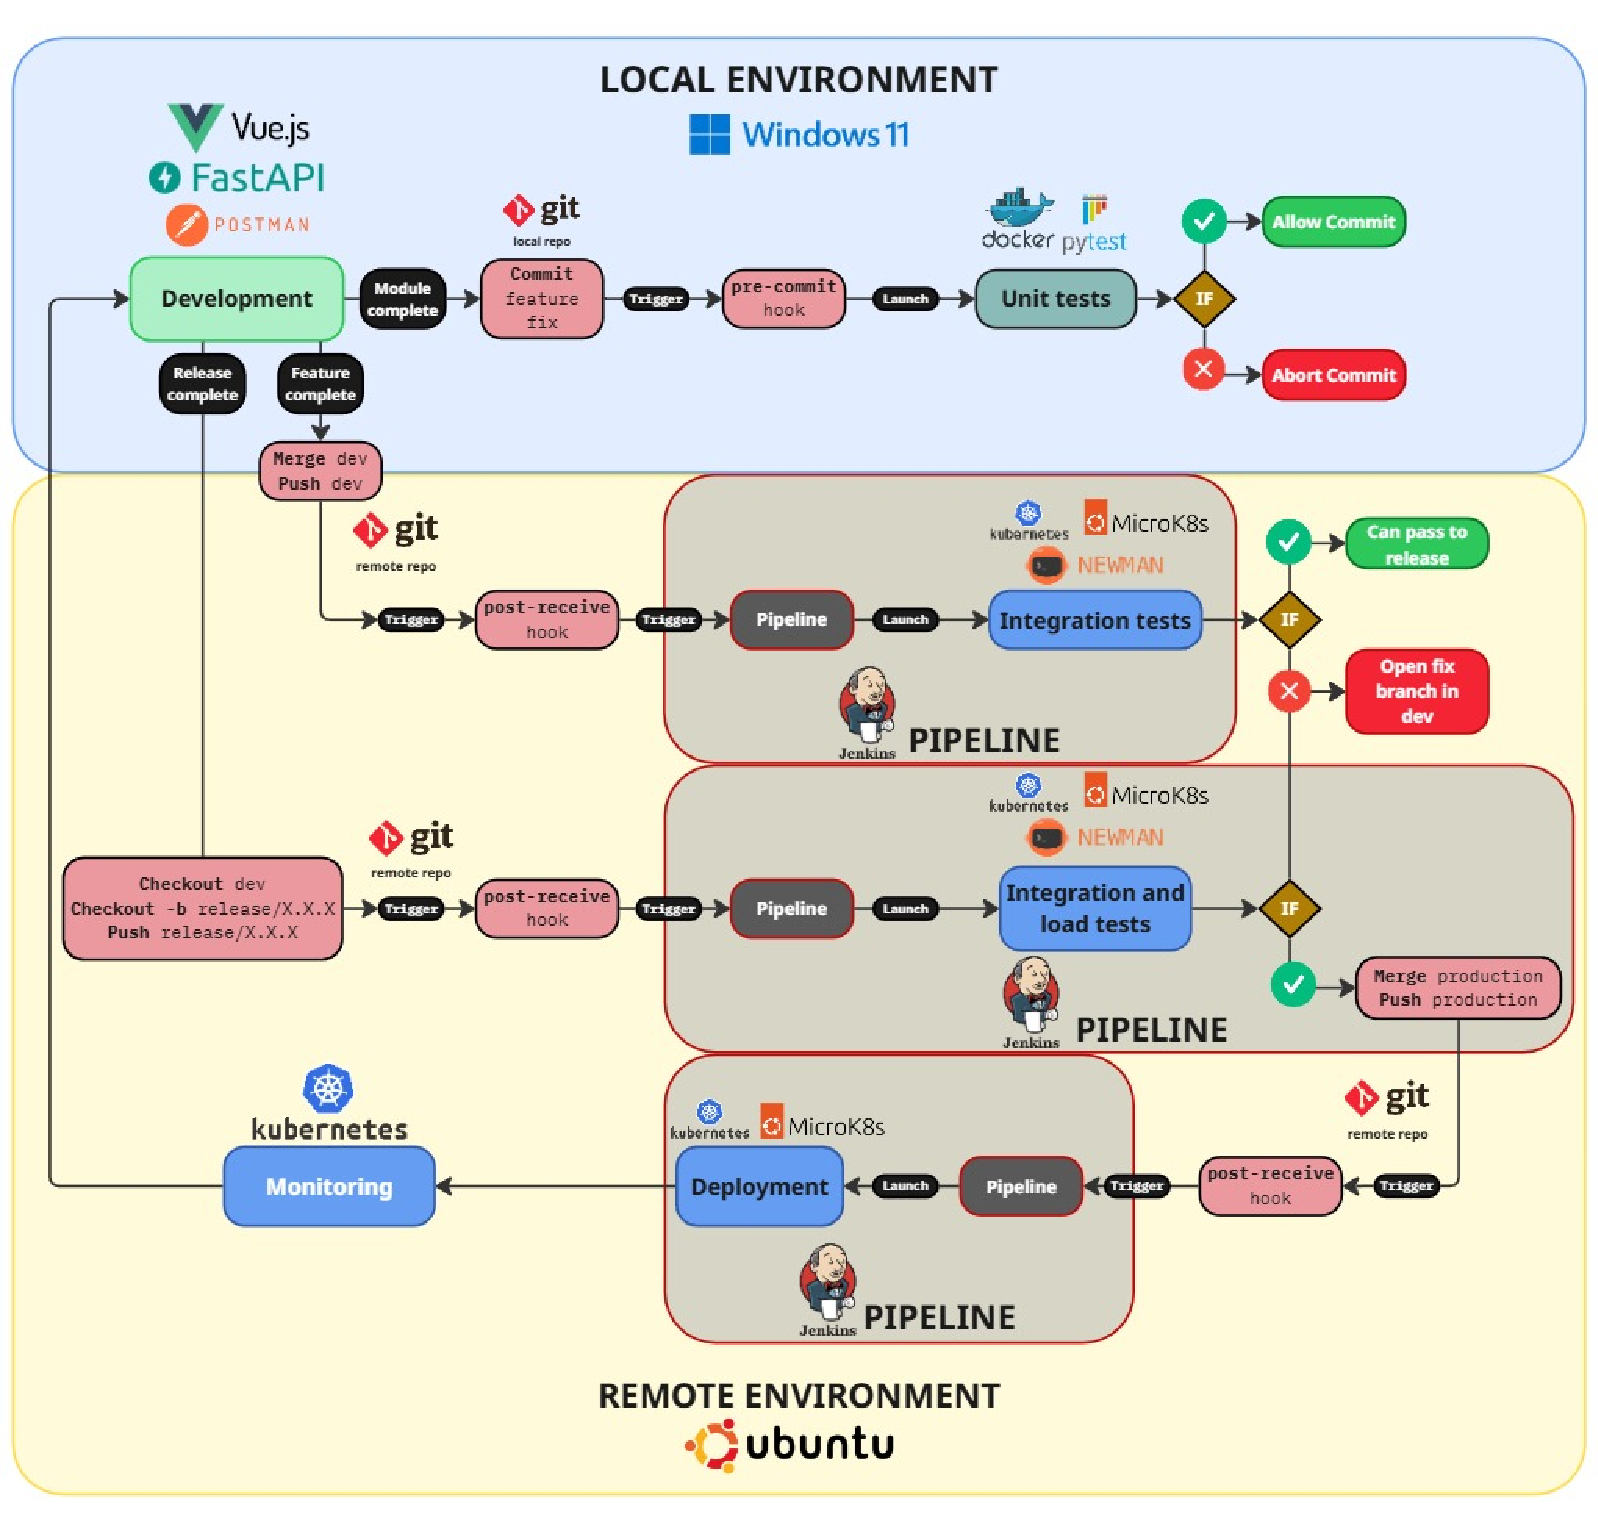
\includegraphics[width=1\linewidth]{Devops/imgs/DEVOPS.pdf}
    \caption{CI/CD Complete Pipeline.}
    \label{fig:pipeline}
\end{figure}

\clearpage

\section{Complete developer workflow}

\subsection{Local Development and Unit Tests}

\begin{itemize}
    \item Developers work on \texttt{feature} branches derived from \texttt{dev}.
    \item A \textbf{local pre-commit hook} runs all unit tests using \texttt{pytest} within a Docker container before any changes are committed.
    \item The commit is only allowed if all unit tests pass successfully.
    \item A commit message template is used to ensure that commit messages are clear, consistent, and informative.
\end{itemize}

\subsection{Local Integration Tests}

\begin{itemize}
    \item \textbf{Integration tests} are executed locally \textbf{before pushing} to the remote repository. This allows developers to catch integration issues early and ensures that the integration tests are well written.
\end{itemize}

\subsection{Completion of a feature and integration tests}

\begin{itemize}
    \item A completed feature branch is \textbf{merged into \texttt{dev}}.
    \item The \texttt{dev} branch is then \textbf{pushed to the remote repository}, triggering automatic integration tests. 
    \begin{itemize}
        \item If they fail, the developer can create a \texttt{fix} branch from \texttt{dev} and then merge and push to \texttt{dev} (more suitable for fixes that require more commits), or he can fix locally and push directly to \texttt{dev} (more suitable for a quick fix).
    \end{itemize}
\end{itemize}

\subsection{Completion of a release, load tests and automatic deployment}

\begin{itemize}
    \item Once a group of features have been tested and are considered ready to be released in production, a developer \textbf{creates and checks out to a \texttt{release/X.X.X} branch}.
    \item This \texttt{release/X.X.X} branch is then \textbf{pushed to the remote repository}, triggering automatic integration and load tests. 
    \begin{itemize}
        \item If they succeed, the \texttt{release/X.X.X} branch is automatically merged to \texttt{production} and the system is automatically deployed.
        \item If they fail, the developer can \textit{cry in a corner because the VM sucks} open a fix branch.
    \end{itemize}
\end{itemize}    

\subsection{Post-deployment and monitoring}
\begin{itemize}
    \item The developers can monitor the state of the Kubernetes cluster using the included \textbf{dashboard}, which also shows resource usage and performance metrics for each pod.
    \item The developers can always visualize a complete report of each series of integration and load tests, which is automatically generated by Newman, using the Jenkins interface. This is particularly useful to troubleshoot in case of failure.
\end{itemize}

\section{Jenkins automation script}

The automation of the pipeline is made possible by a \texttt{Jenkinsfile} included in the Git repository, which executes specific actions based on the branch that triggered the script.

\begin{itemize}
    \item \textbf{If branch is \texttt{fix} or \texttt{feature}}:
    \begin{itemize}
        \item Jenkins takes \textbf{no action}.
    \end{itemize}
    \item \textbf{If branch is \texttt{dev}}:
    \begin{itemize}
        \item The Docker images of the microservices are built with tag \textit{test} and pushed to DockerHub.
        \item Kubernetes uses the images from DockerHub and the deployment specifications to deploy the application in the test environment (it has its specific namespace, so the test and production resources are separated).
        \item \textbf{Integration tests} are run using \textbf{Newman} (for Postman collections).
        \item If tests fail the pipeline fails alerting the developers.
        \item If tests pass the pipeline completes successfully.
        \item In any case the deployment is eliminated to release the resources.
    \end{itemize}
    \item \textbf{If branch is \texttt{release}}:
    \begin{itemize}
        \item The Docker images of the microservices are built with tag \textit{test} and pushed to DockerHub.
        \item Kubernetes uses the images from DockerHub and the deployment specifications to deploy the application in the test environment (it has its specific namespace, so the test and production resources are separated).
        \item \textbf{Integration and load tests} are run using \textbf{Newman}.
        \item If tests fail the pipeline fails alerting the developers.
        \item If tests pass:
        \begin{itemize}
            \item Jenkins performs a \textbf{fast-forward merge from \texttt{release} to \texttt{production}}. This simulates a pre-receive hook's function as Jenkins acts as the authorized pusher.
            \item Jenkins then \textbf{pushes the changes to the \texttt{production} branch}, triggering another instance of the pipeline for which the branch is \texttt{production}.
        \end{itemize}
        \item In any case the deployment is eliminated to release the resources.
    \end{itemize}
    \item \textbf{If branch is \texttt{production}}:
    \begin{itemize}
        \item The Docker images of the microservices are built with tag \textit{prod} and pushed to DockerHub.
        \item Kubernetes uses the images from DockerHub and the deployment specifications to deploy the application in the production environment (it has its specific namespace, so the test and production resources are separated).
        \begin{itemize}
            \item Since the production deployment is always up, a new deployment triggers a rolling upgrade that minimizes downtime. 
        \end{itemize}
    \end{itemize}
\end{itemize}